\section{Sortie du programme}
\begin{figure}[h]
    \centering
    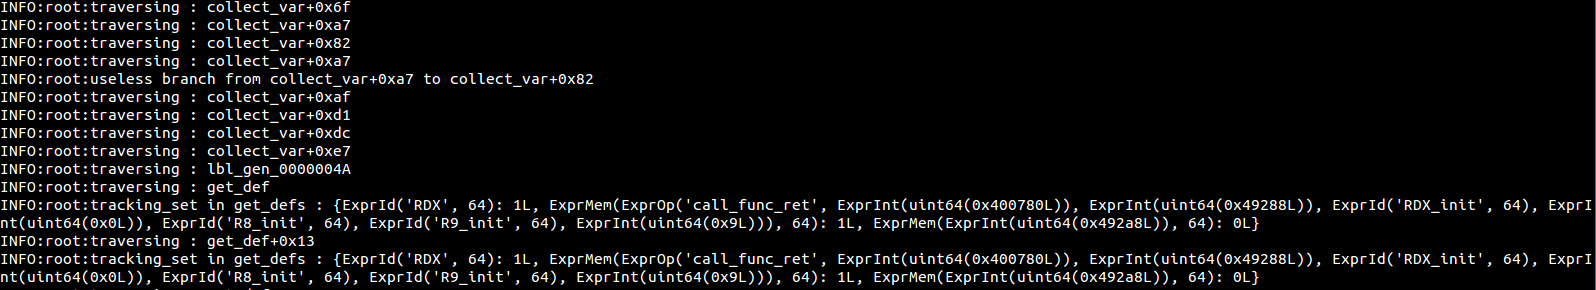
\includegraphics[scale=0.5]{tracking-set.png}
    \caption{Représentation de l'attribut tracking\_set (affichage de debug).}
    Chaque emplacement est associé à un identifiant d'allocation.
\end{figure}

\section{Graphes}

\begin{figure}[h]
    \centering
    \begin {lstlisting}[frame=single]
int *global = NULL;

static void e(void) {
    printf("Test.\n");
}

static void g(int fd, int fd2, int fd3) {
    close(fd);
    for (int i = 0; i < (fd + fd2 + fd3); i ++)
        e();
}

void f(void) {
    int fd = open("file", O_RDONLY);
    g(fd, fd + 1, fd + 2);
    int a = a + 1;
    int *b = malloc(sizeof(int));
    int *i = malloc(sizeof(int));
    for (int i = 0; i < 10; i++) {
        printf("foo : %p\n", b);
        a += 2;
    }
    free(b);
    int *c = i;
    int *d = i;
    global = d;
    printf("%d%s%p", a, "f\n", c);
    printf("%d%s%p", a, "f\n", d);
    printf("%d%s%p", a, "f\n", global);
}

int main(void)
{
    while (1) {
      for (int i = 0; i < 50; i++) {
            if (malloc(sizeof(int)))
                f();
            else
                g(i, i+1, i+2);
      }
    }
    return 0;
}
    \end{lstlisting}
    \caption{Programme 1.}
\end{figure}


\begin{figure}[h]
    \centering
    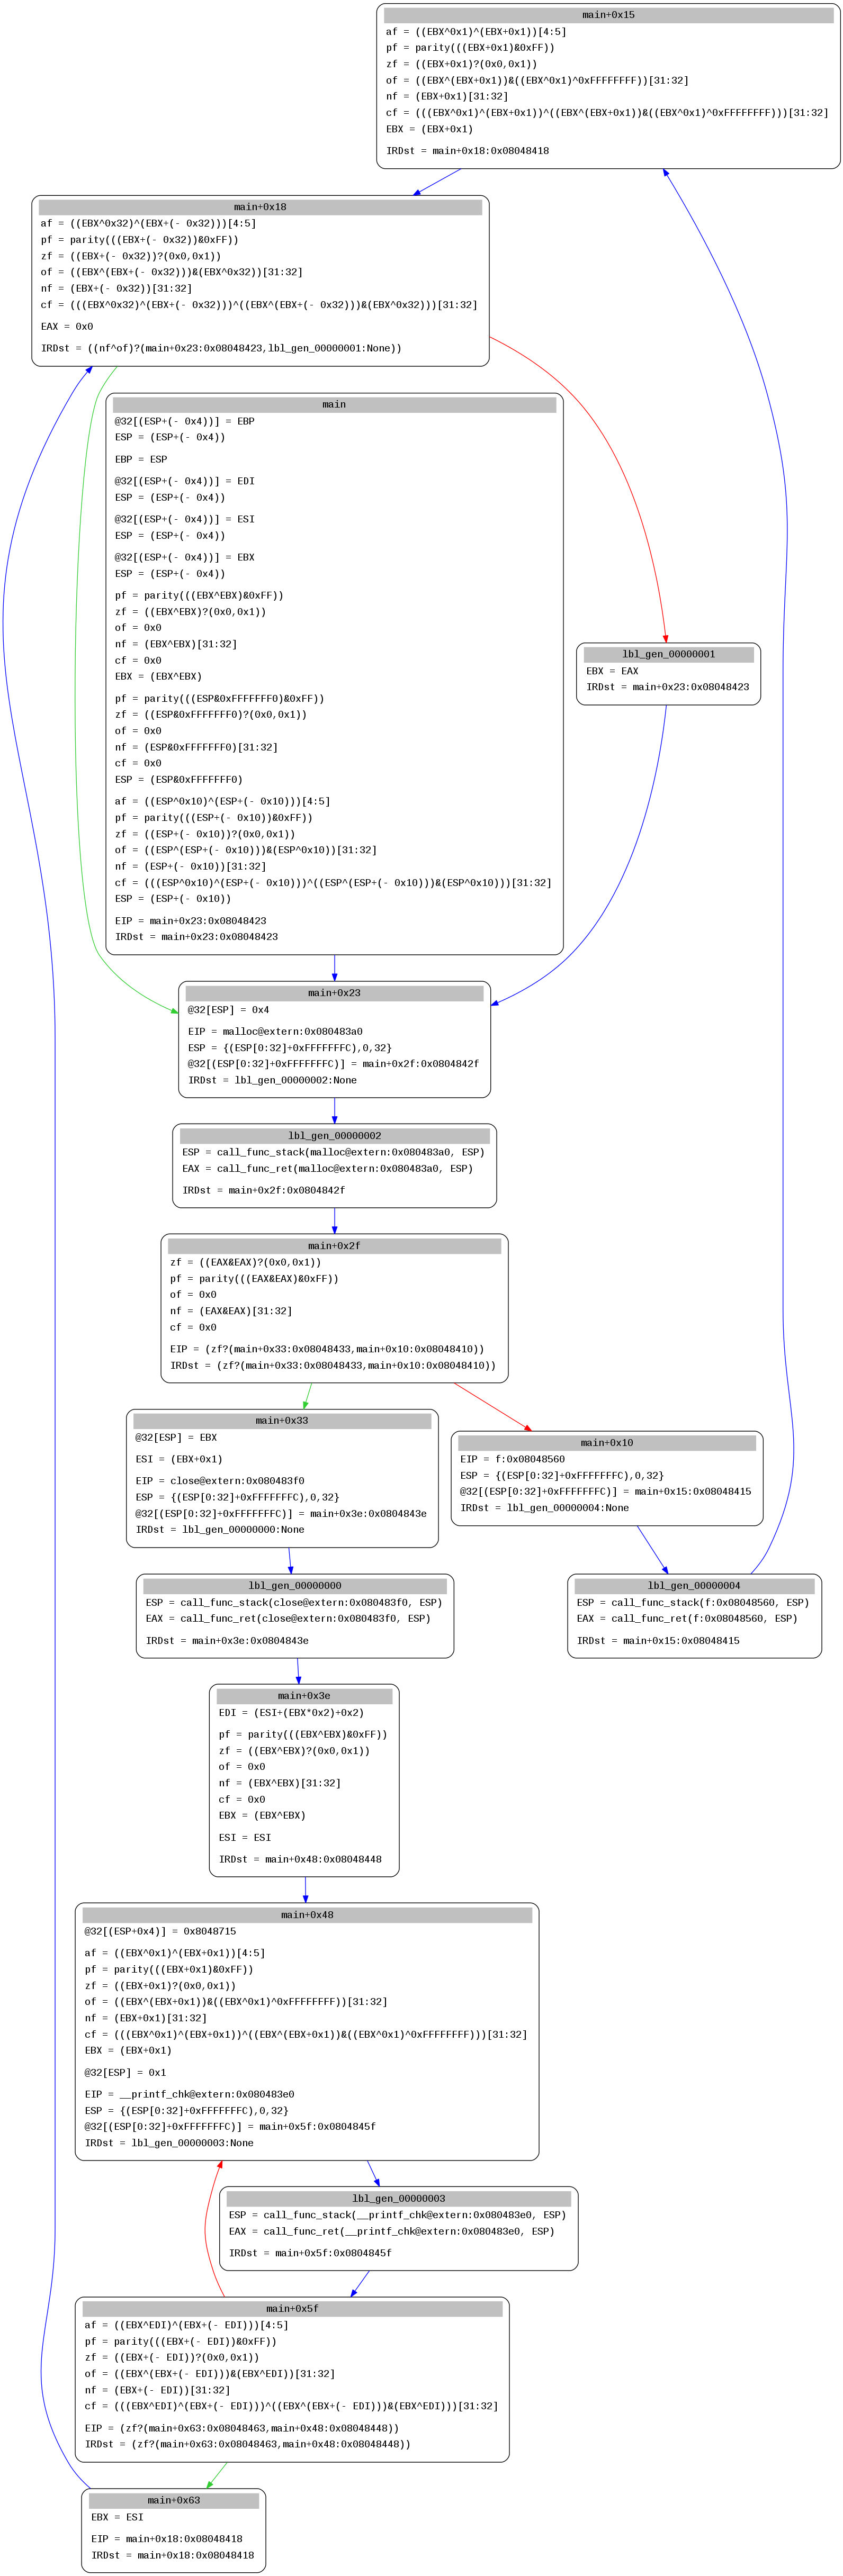
\includegraphics[scale=0.125]{simple-graph.png}
    \caption{Graphe associé au programme 1}
\end{figure}
\begin{figure}[h]
    \centering
    \begin {lstlisting}[frame=single]
allocation:
g_malloc0@extern
g_malloc0_n@extern
g_malloc@extern
g_malloc_n@extern
free:
g_free@extern
    \end{lstlisting}
    \caption{Fonction traquées pour le logiciel evince. }
    Fichier de configuration contenant les fonctions traquées pour le logiciel
evince sous Linux (Ubuntu 14.10).
\end{figure}

%\begin{figure}[h]
%    \centering
%    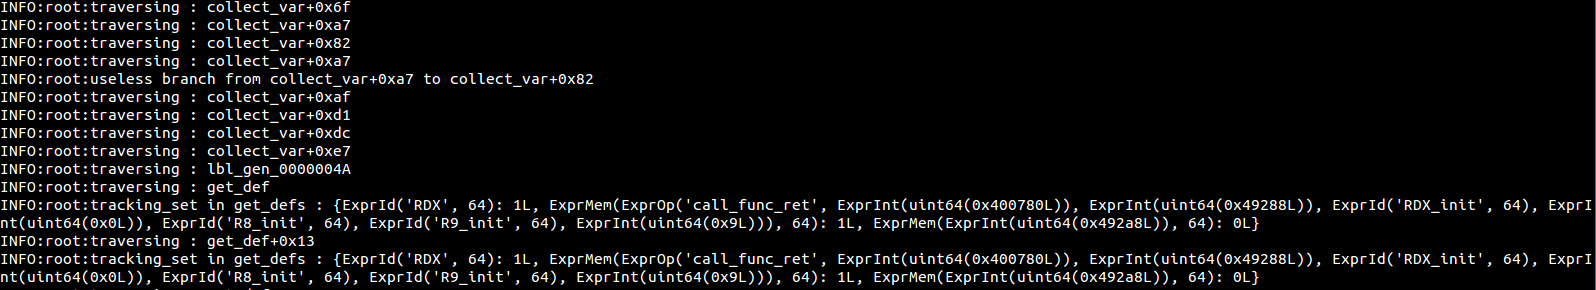
\includegraphics[scale=0.001]{tracking-set.png}
%    \caption{Graphe d'un petit projet de première année du cyle ingénieur.}
%\end{figure}

